\documentclass{beamer}
%\documentclass[12pt]{beamer}
\usepackage{graphicx}
\usepackage[utf8]{inputenc}
\usetheme{Madrid}
\usepackage{verbatim}
\usepackage{subcaption}
\usepackage{amsmath}
\usepackage{hyperref}
\usepackage{multirow}

\title{Sorting: Quicksort and Merge sort}
\author[1305050,1305067,1405069]{\alert{Zaki Tahmeed, H.M.Mutammil Galib and Faiyaz Rashid Nabil}}
\institute[CSE,BUET]{Bangladesh University of Engineering and Technology}
\date{\today}

\logo{
\includegraphics[height=1cm]{buet_logo.png}}

 \AtBeginSection[]
 {
   \begin{frame}
     \frametitle{Table of Contents}
     \tableofcontents[currentsection]
   \end{frame}
 }

\begin{document}

\frame{\titlepage}

 \section{Sorting}
 
 \begin{frame}{Sorting}
 Sorting is any process of arranging items systematically and in a sequence ordered by some criterion.The most common uses of sorting are:
  \begin{itemize}
   \item<2->  making lookup or search efficient.
   \item<3-> making merging of sequences efficient.
   \item<4-> enable processing of data in a defined order.
  \end{itemize}
 \end{frame}
 
 \section{Sorting Algorithm}
 
 \begin{frame}{Sorting Algorithm}
A sorting algorithm is an algorithm that puts elements of a list in a certain order. The most frequently used orders are numerical order and lexicographical order. Efficient sorting is important for optimizing the efficiency of other algorithms that require input data to be in sorted lists.Some popular sorting algorithms are:
	\begin{itemize}
		\item<2-> Insertion Sort
		\item<3-> Selection sort
		\item<4-> Heapsort
		\item<5-> Merge Sort
		\item<6-> Quicksort
		\item<7-> Bubble sort
	\end{itemize}
\end{frame}

\section{Divide and Conquer}

\begin{frame}{Divide and Conquer}
		Divide and conquer is an algorithm design paradigm.The concept of Divide and Conquer involves three steps:\pause
		\begin{itemize}
			\item	Divide the problem into multiple small problems.\pause
			\item  	Conquer the subproblems by solving them. The idea is to break down the problem into atomic subproblems, where they are actually solved.\pause
			\item   Combine the solutions of the subproblems to find the solution of the actual problem.\pause
		\end{itemize}
	    \begin{examples}
	    The divide-and-conquer technique is the basis of efficient algorithms for many problems, such as sorting (e.g., quicksort, merge sort), multiplying large numbers (e.g., the Karatsuba algorithm), finding the closest pair of points, syntactic analysis (e.g., top-down parsers), and computing the discrete Fourier transform (FFT).
	    \end{examples}   
\end{frame}

\section{Quicksort}

 \begin{frame}{Quicksort}
 	    
 	     \begin{block}{Introduction}
 		   \begin{itemize}
 		\item<2-> Quicksort is a divide-and-conquer algorithm.
 		\item<3-> Quick sort is a highly efficient sorting algorithm and is based on partitioning of array of data into smaller arrays. 
 		\item<4-> It was Developed by British computer scientist Tony Hoare in 1959 and published in 1961.
 		\item<5-> It is an in-place sorting algorithm, requiring small additional amounts of memory to perform the sorting.
 		\item<6-> When implemented well, it can be somewhat faster than merge sort and about two or three times faster than heapsort.
           \end{itemize}
        \end{block}
  
 \end{frame}
 
  \begin{frame}{Quicksort}
 	   
 	    \begin{block}{Procedure}
 	    \begin{itemize}
 		\item<2->The array of elements is divided into parts repeatedly until it is not possible to divide it further.
 		\item<3-> It works by selecting a 'pivot' element from the array and partitioning the other elements into two sub-arrays.
 		\item<4-> In the first sub-array, all elements are less than or equal to the pivot value.
 		\item<5->  In the second sub-array, all elements are greater than or equal to the pivot value.
 		\item<6-> The sub-arrays are then sorted recursively. 
 			\end{itemize}
 		\end{block}

  \end{frame}
 
 \begin{frame}{Quicksort}
 \begin{figure}[h]
 	\centering
 	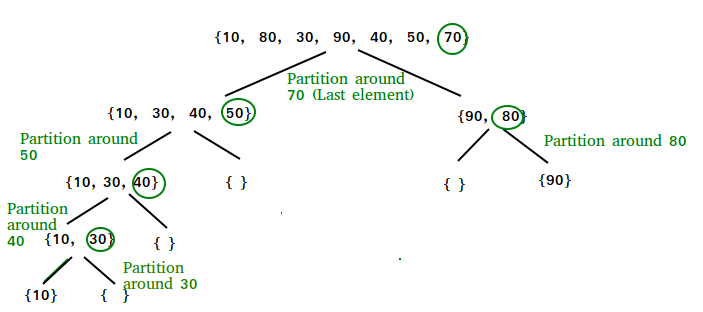
\includegraphics[scale=0.5]{QuickSort2.png}
 	\label{fig:1}
 	\caption{Quicksort Algorithm}
 \end{figure}
 \end{frame}

\begin{frame}{Time Complexity}
	
	\begin{block}{Best-case Analysis}
		In the most balanced case, each time we perform a partition we divide the list into two nearly equal pieces. This means each recursive call processes a list of half the size.\pause 
		
		Consequently, we can make only $log_2 n$ nested calls before we reach a list of size $1$. This means that the depth of the call tree is  $log_2 n$ . But no two calls at the same level of the call tree process the same part of the original list. \pause
		
		Thus, each level of calls needs only $O(n)$ time all together (each call has some constant overhead, but since there are only $O(n)$ calls at each level, this is subsumed in the $O(n)$ factor). The result is that the algorithm uses only \alert{$O(n log n)$} time.	
	\end{block}
	
\end{frame}

\begin{frame}{Time Complexity}
    
    \begin{alertblock}{Worst-case Analysis}
    	The most unbalanced partition occurs when one of the sublists returned by the partitioning routine is of size $n - 1$.This may occur if the pivot happens to be the smallest or largest element in the list.\pause
    	
    	If this happens repeatedly in every partition, then each recursive call processes a list of size one less than the previous list. Consequently, we can make $n - 1$ nested calls before we reach a list of size $1$.\pause 
    	
    	This means that the call tree is a linear chain of $n - 1$ nested calls. The $ith$ call does $O(n - i)$ work to do the partition, and $\sum_{i=0}^{n} (n-i) = O(n^2)$, so in that case quicksort takes \alert{$O(n^2)$} time.
    \end{alertblock}\pause
   
    \begin{block}{Average-case Analysis}
    To sort an array of $n$ distinct elements, quicksort takes \alert{$O(n log n)$} time in expectation, averaged over all $n!$ permutations of $n$ elements with equal probability. 	
    \end{block}

\end{frame}

%Merge sort
 \section{Merge sort}
\begin{frame}{Merge sort}
		\begin{block}{Introduction}
			\begin{itemize}
			\item<2->  Merge sort is an efficient, general-purpose, and comparison-based sorting algorithm. 
			\item<3-> Merge sort is a divide and conquer algorithm that was invented by John von Neumann in 1945. 
			\item<4->A detailed description and analysis of bottom-up merge sort appeared in a report by Goldstine and von Neumann as early as 1948.
			\end{itemize}
		\end{block}
\end{frame}	  

\begin{frame}{Merge sort}  
	     \begin{block}{Procedure}
	    	\begin{itemize}
	    	\item<2->The elements are split into two sub-arrays $(n/2)$ again and again until only one element is left.
	    	\item<3-> Merge sort uses additional storage for sorting the auxiliary array.
	    	\item<4->  Merge sort uses three arrays where two are used for storing each half, and the third external one is used to store the final sorted list by merging other two and each array is then sorted recursively.
	    	\item<5->  At last, the all sub arrays are merged to make it ‘n’ element size of the array. 
	    	\end{itemize}
	    \end{block}
\end{frame}

\begin{frame}{Merge sort}
	\begin{figure}[h]
		\centering
		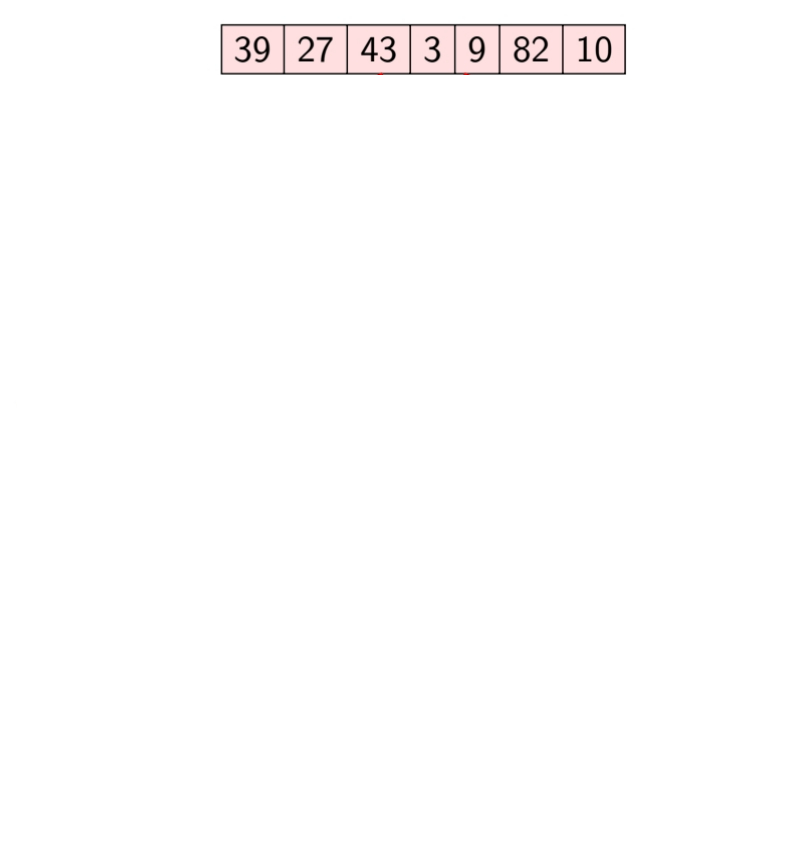
\includegraphics[scale=0.24]{IKEHS1.jpg}
		\label{fig:2}
		\caption{Merge sort Algorithm}
	\end{figure}
\end{frame}

\begin{frame}{Merge sort}
	\begin{figure}[h]
		\centering
		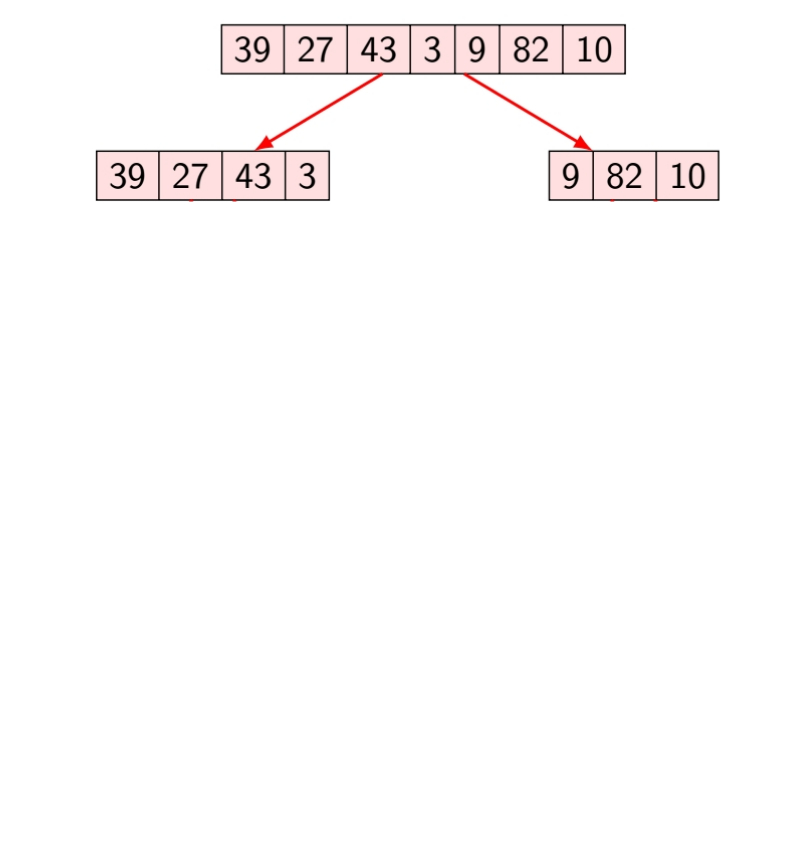
\includegraphics[scale=0.24]{IKEHS2.jpg}
		\label{fig:2}
		\caption{Merge sort Algorithm}
	\end{figure}
\end{frame}

\begin{frame}{Merge sort}
	\begin{figure}[h]
		\centering
		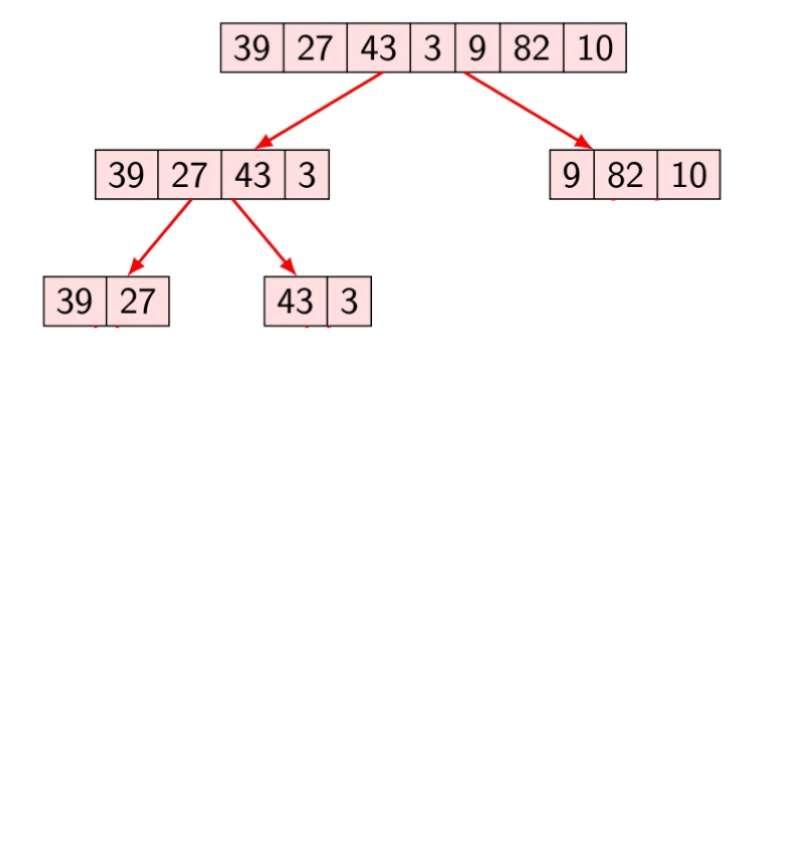
\includegraphics[scale=0.24]{IKEHS3.jpg}
		\label{fig:2}
		\caption{Merge sort Algorithm}
	\end{figure}
\end{frame}

\begin{frame}{Merge sort}
	\begin{figure}[h]
		\centering
		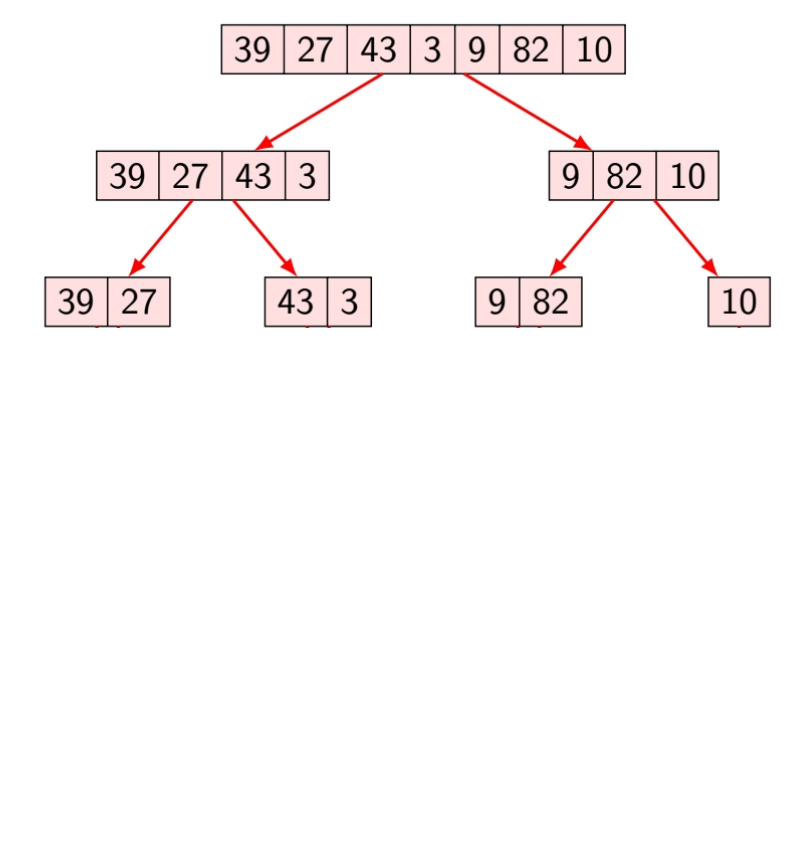
\includegraphics[scale=0.24]{IKEHS4.jpg}
		\label{fig:2}
		\caption{Merge sort Algorithm}
	\end{figure}
\end{frame}

\begin{frame}{Merge sort}
	\begin{figure}[h]
		\centering
		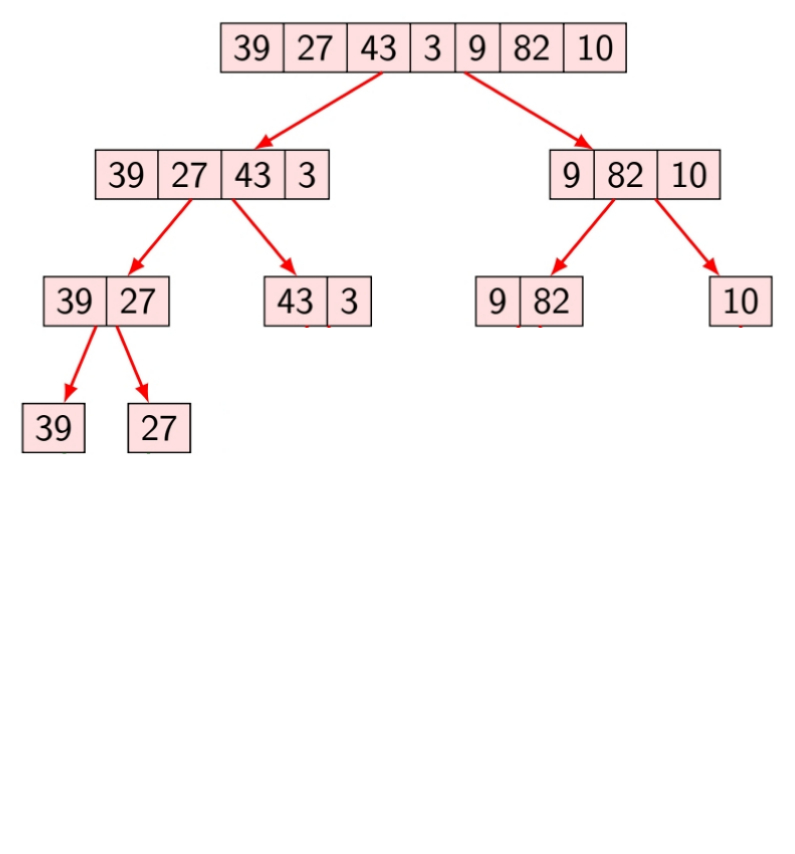
\includegraphics[scale=0.24]{IKEHS5.jpg}
		\label{fig:2}
		\caption{Merge sort Algorithm}
	\end{figure}
\end{frame}

\begin{frame}{Merge sort}
	\begin{figure}[h]
		\centering
		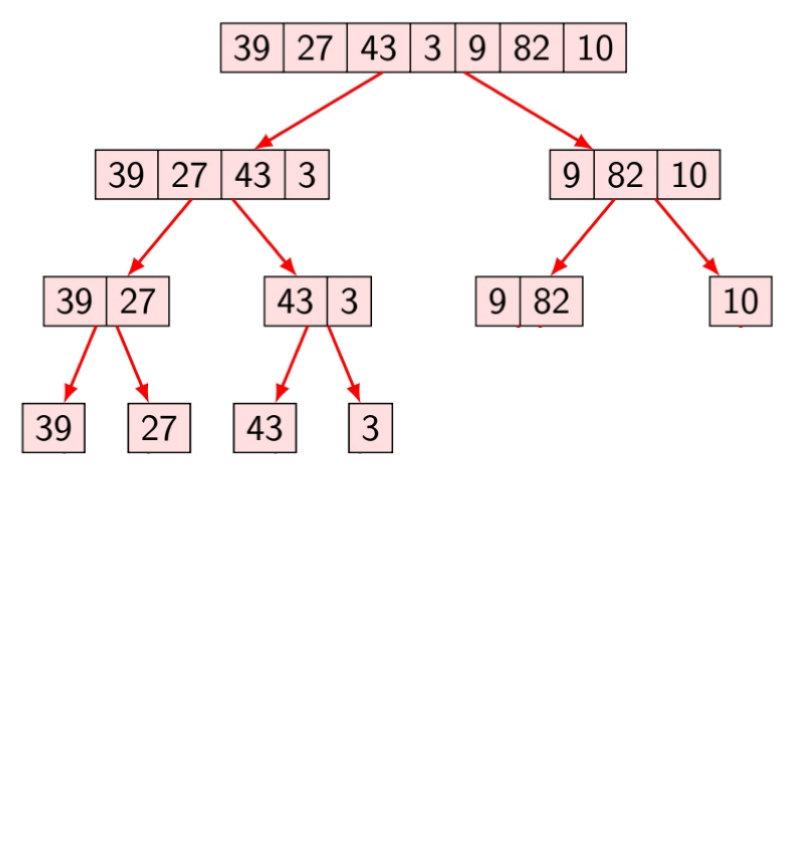
\includegraphics[scale=0.24]{IKEHS6.jpg}
		\label{fig:2}
		\caption{Merge sort Algorithm}
	\end{figure}
\end{frame}

\begin{frame}{Merge sort}
	\begin{figure}[h]
		\centering
		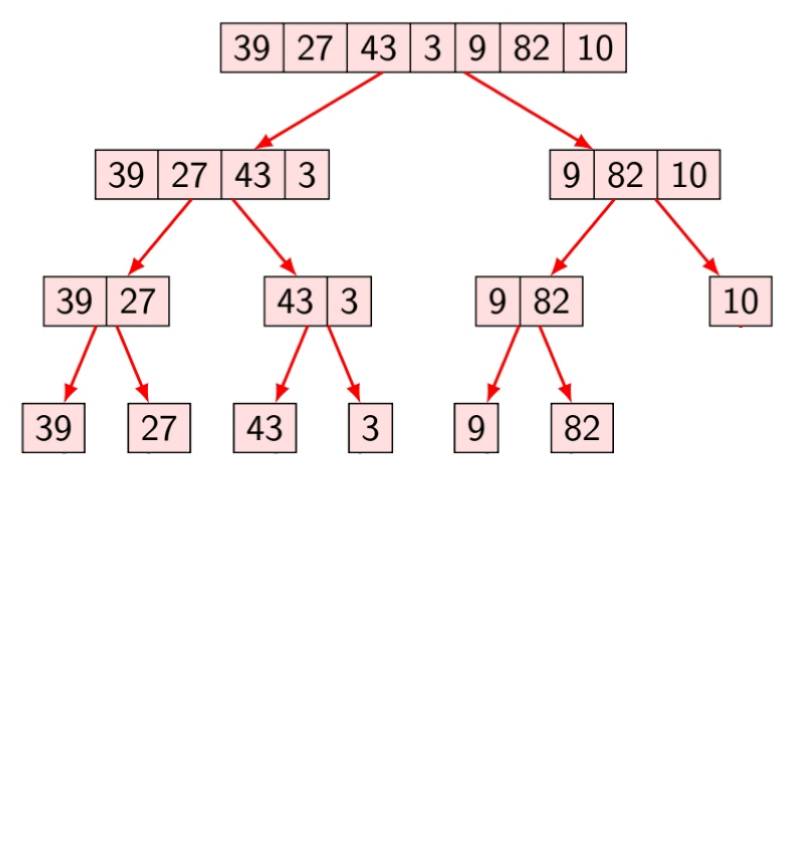
\includegraphics[scale=0.24]{IKEHS7.jpg}
		\label{fig:2}
		\caption{Merge sort Algorithm}
	\end{figure}
\end{frame}

\begin{frame}{Merge sort}
	\begin{figure}[h]
		\centering
		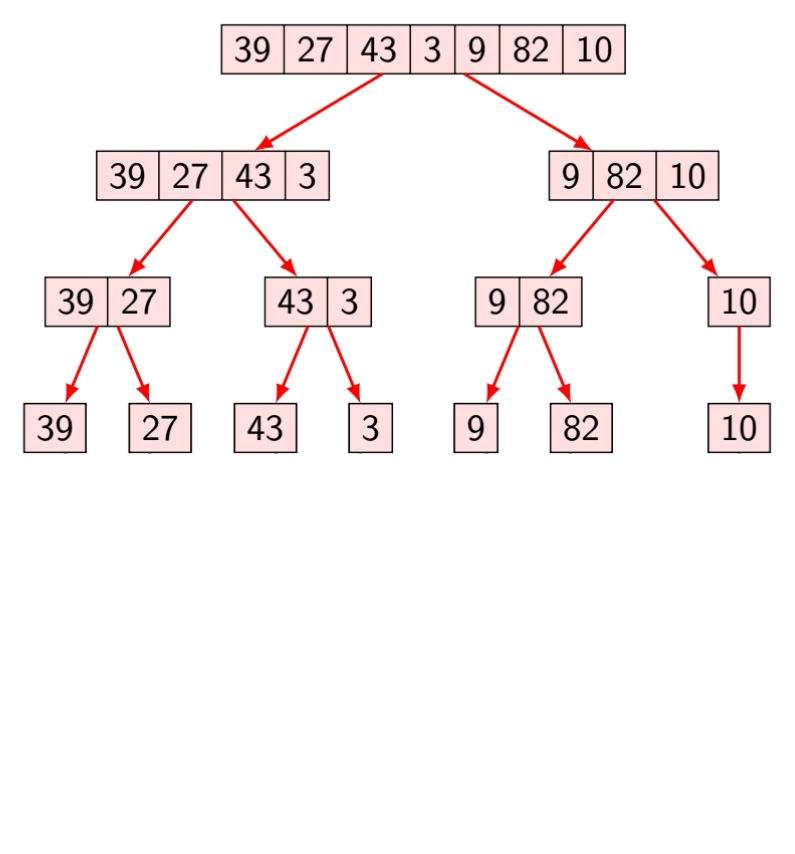
\includegraphics[scale=0.24]{IKEHS8.jpg}
		\label{fig:2}
		\caption{Merge sort Algorithm}
	\end{figure}
\end{frame}

\begin{frame}{Merge sort}
	\begin{figure}[h]
		\centering
		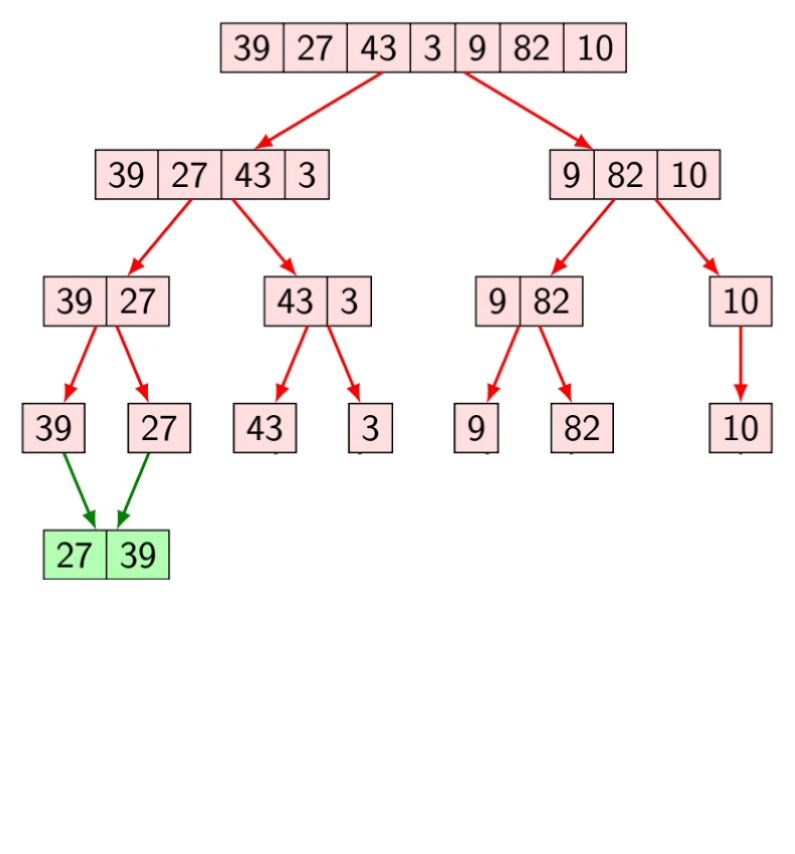
\includegraphics[scale=0.24]{IKEHS9.jpg}
		\label{fig:2}
		\caption{Merge sort Algorithm}
	\end{figure}
\end{frame}

\begin{frame}{Merge sort}
	\begin{figure}[h]
		\centering
		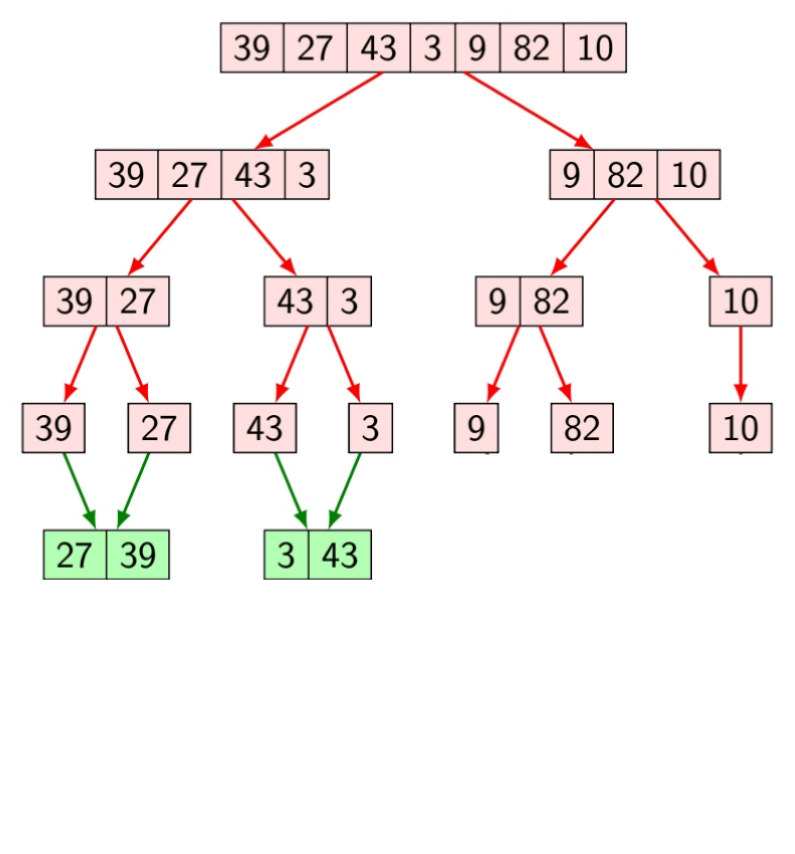
\includegraphics[scale=0.24]{IKEHS10.jpg}
		\label{fig:2}
		\caption{Merge sort Algorithm}
	\end{figure}
\end{frame}

\begin{frame}{Merge sort}
	\begin{figure}[h]
		\centering
		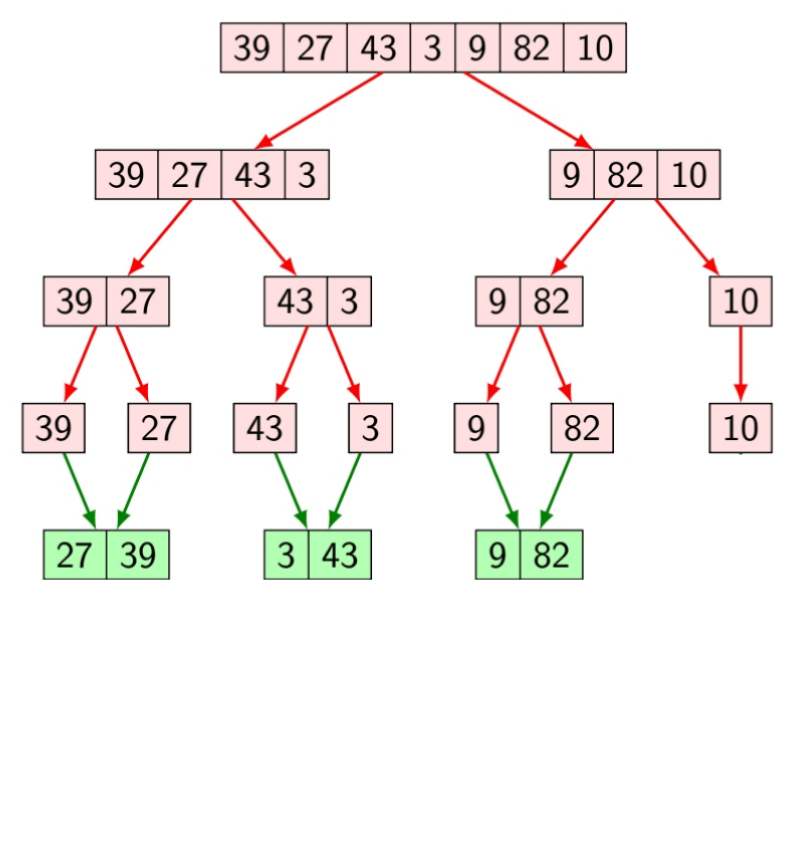
\includegraphics[scale=0.24]{IKEHS11.jpg}
		\label{fig:2}
		\caption{Merge sort Algorithm}
	\end{figure}
\end{frame}

\begin{frame}{Merge sort}
	\begin{figure}[h]
		\centering
		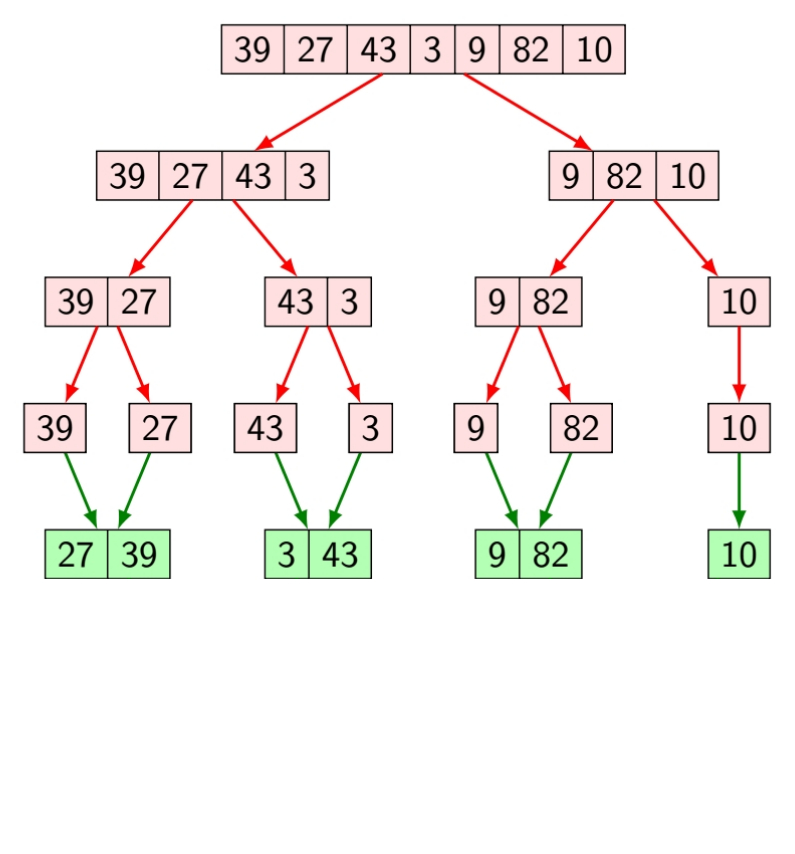
\includegraphics[scale=0.24]{IKEHS12.jpg}
		\label{fig:2}
		\caption{Merge sort Algorithm}
	\end{figure}
\end{frame}

\begin{frame}{Merge sort}
	\begin{figure}[h]
		\centering
		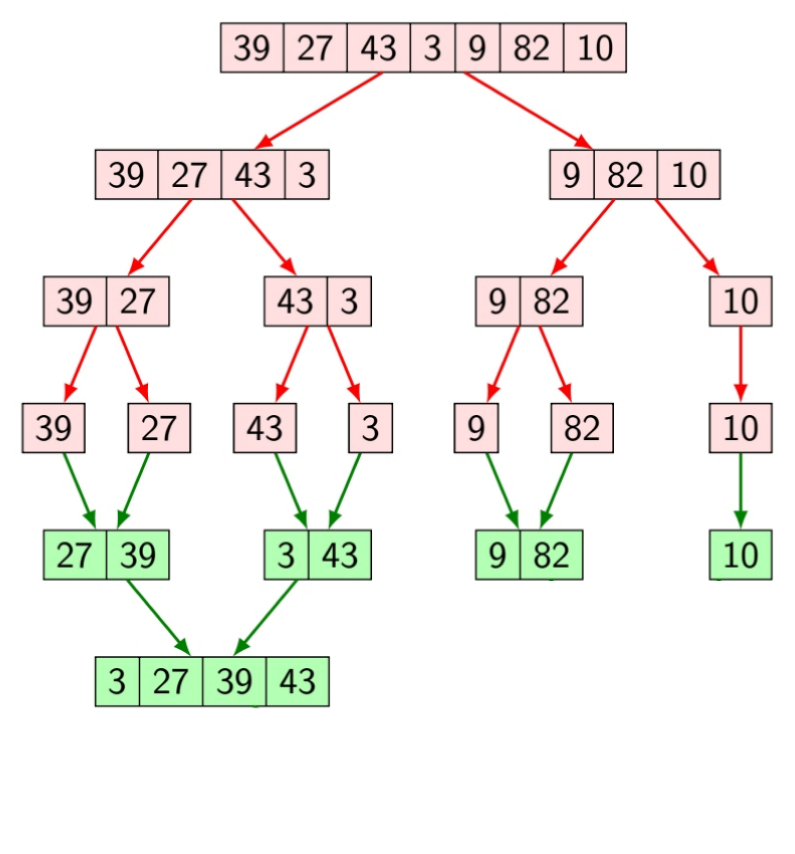
\includegraphics[scale=0.24]{IKEHS13.jpg}
		\label{fig:2}
		\caption{Merge sort Algorithm}
	\end{figure}
\end{frame}

\begin{frame}{Merge sort}
	\begin{figure}[h]
		\centering
		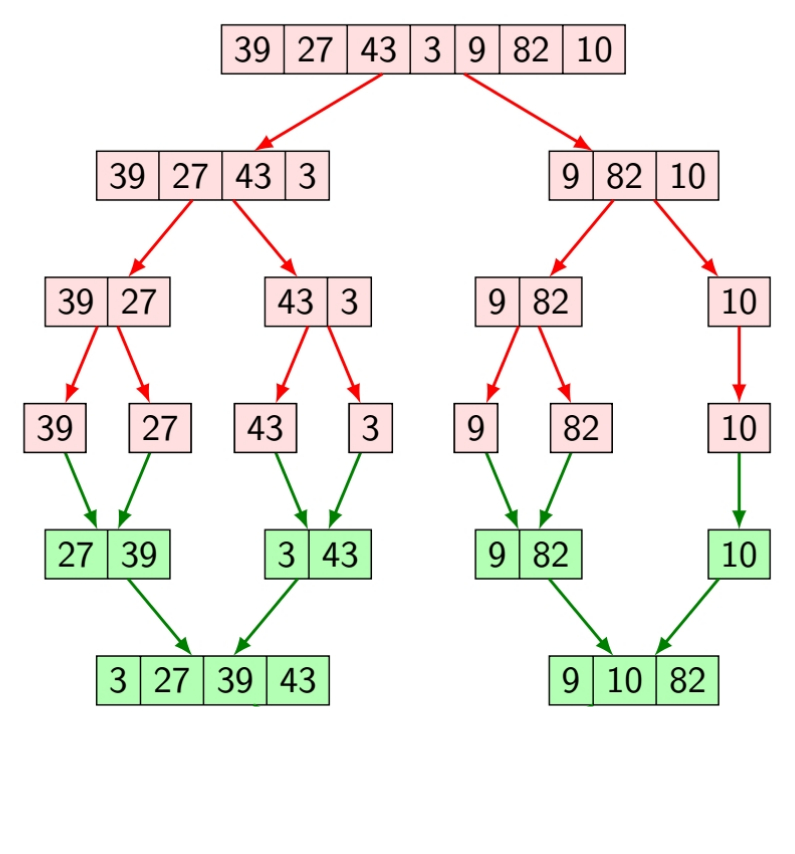
\includegraphics[scale=0.24]{IKEHS14.jpg}
		\label{fig:2}
		\caption{Merge sort Algorithm}
	\end{figure}
\end{frame}

\begin{frame}{Merge sort}
	\begin{figure}[h]
		\centering
		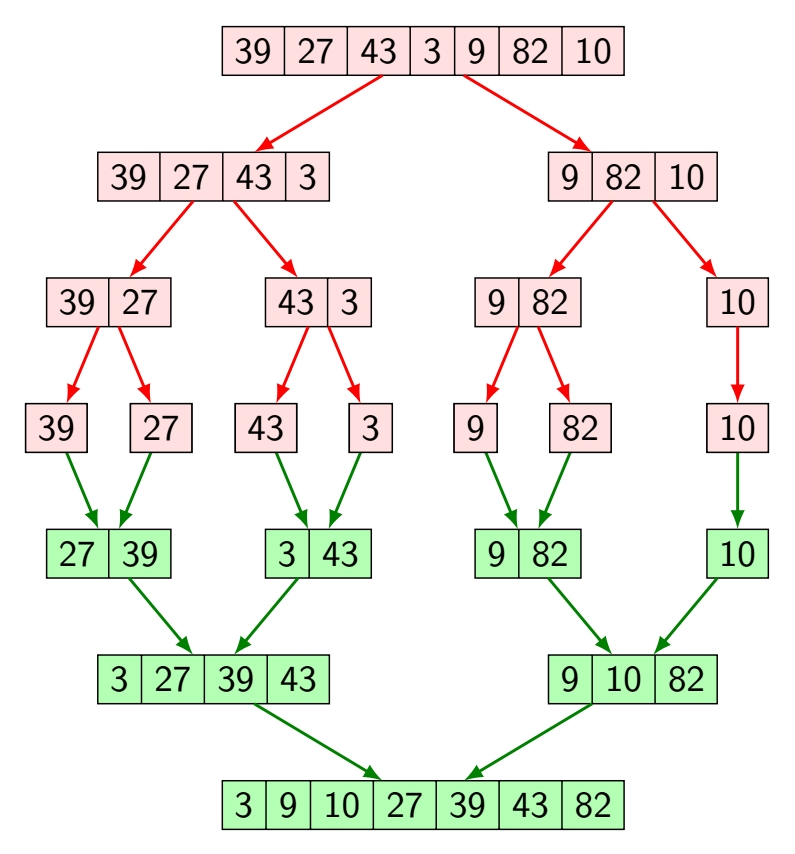
\includegraphics[scale=0.24]{IKEHS15.jpg}
		\label{fig:2}
		\caption{Merge sort Algorithm}
	\end{figure}
\end{frame}

\begin{frame}{Time Complexity}
	
	Time complexity of Merge Sort is  \alert{$O(n log n)$} in all $3$ cases (worst, average and best) as merge sort always divides the array into two halves and takes linear time to merge two halves.\pause

	Whenever we divide a number into half in every step, it can be represented using a logarithmic function ($log n$) and the number of steps can be represented by $log n + 1$(at most).\pause

	Also, we perform a single step operation to find out the middle of any subarray which requires $O(1)$ time.\pause
	
	And to merge the subarrays, made by dividing the original array of n elements, a running time of $O(n)$ will be required.\pause
	
	Hence the total time for merge Sort function will become $n(log n + 1)$, which gives us a time complexity of \alert{$O(nlog n)$}.
	
\end{frame}

\section{Comparison}
  
  \begin{frame}{Comparison}
	    
	    \centering
	    \begin{tabular}{|c|c|c|}
		\hline
		 Basis for  & \multirow{2}{*}{Quicksort} & \multirow{2}{*}{Merge sort} \\
		 Comparison & & \\
	    \hline
	    \hline
	     \onslide<2->{Worst case}  &  \onslide<2->{\multirow{2}{*}{$O(n^2)$}} &  \onslide<2->{\multirow{2}{*}{ $O(nlogn)$}} \\ 
		  \onslide<2->{complexity} & & \\
		\hline
		 \onslide<3->{\multirow{2}{*}{Efficiency}} &  \onslide<3->{Inefficient for}  &  \onslide<3->{More efficient for}\\
		&  \onslide<3->{larger arrays} &  \onslide<3->{larger arrays} \\
		\hline
	      \onslide<4->{Sorting method} &  \onslide<4->{Internal} &	 \onslide<4->{External} \\
		\hline
		 \onslide<5->{Preferred for} &   \onslide<5->{Arrays} &  \onslide<5->{Linked Lists} \\
		\hline
		 \onslide<6->{Speed of}  &  \onslide<6->{It works faster on}  &  \onslide<6->{It has a consistent speed} \\
	    \onslide<6-> {execution} & \onslide<6->{small data set} &  \onslide<6-> {on any size of data}  \\
		\hline 
		 \onslide<7->{Additional storage} &   \onslide<7->{\multirow{2}{*}{Less}} &	 \onslide<7->{\multirow{2}{*}{More}} \\
		 \onslide<7->{space requirement} & & \\
		\hline
		 \onslide<8->{Partition of}  &	 \onslide<8->{An array can be}  &	 \onslide<8-> {An array will be divided} \\
		 \onslide<8->{elements} &  \onslide<8->{ divided into any ratio} &    \onslide<8->{into two sub arrays} \\
		\hline
		\end{tabular}
	 
   \end{frame}

\end{document}